%!TEX program = xelatex
\documentclass[10pt]{beamer}

\usetheme[progressbar=frametitle, noframetitleoffset, block=fill]{m}
%\definecolor{TUMblue}{RGB}{55,55,255}
%\setbeamercolor{alerted text}{fg=TUMblue}

\usepackage{booktabs}
\usepackage[scale=2]{ccicons}

\usepackage{pgfplots}
\usepackage{tikz}
\usepgfplotslibrary{dateplot}
\usepackage{caption}

\newlength\figureheight
\newlength\figurewidth
\DeclareMathOperator{\prox}{prox}
\DeclareMathOperator{\argmin}{argmin}

\title{Stochastic Optimization in Machine Learning}
\subtitle{Case Studies in Nonlinear Optimization}
\date{\today}
\author{F. Bauer \and S. Chambon \and R. Halbig \and S. Heidekrüger \and J. Heuke}
\institute{Technische Universität München}
%\titlegraphic{\hfill
\includegraphics[height=1.5cm]{logo.eps}}

\begin{document}

\maketitle

\plain{
  \begin{quote}
    We're not running out of data anytime soon. It's maybe the only resource that grows exponentially.
    \\
    \flushright{\alert{Andreas Weigend}}
  \end{quote}
  }


\begin{frame}
  \frametitle{Outline}
  \setbeamertemplate{section in toc}[sections numbered]
  \tableofcontents[hideallsubsections]
\end{frame}

\section{Introduction}

  \begin{frame}[t]\frametitle{What is Machine Learning?}
	  	Implementation of autonomously learning software for:
        \begin{itemize}
        	\item Discovery of patterns and relationships in data
        	\item Prediction of future events
        \end{itemize}
        \alert{Examples:}
        \begin{columns}[T]
        	\begin{column}{.25\textwidth}
        		Higgs-Boson\\
        		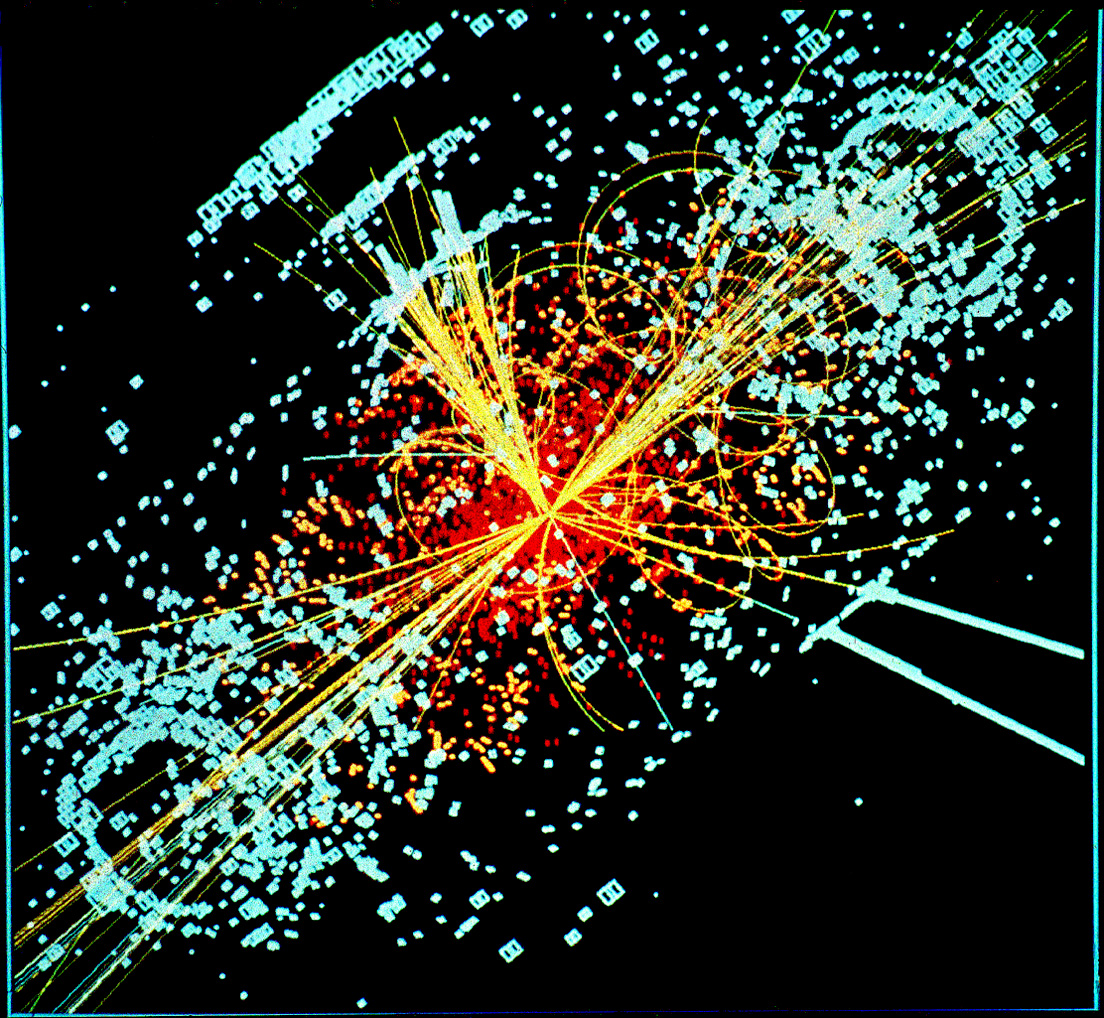
\includegraphics[width = \linewidth]{CMS_Higgs-event.jpg}
        	\end{column}\hfill
        	\begin{column}{.25\textwidth}
        		Compressed Sensing\\
        		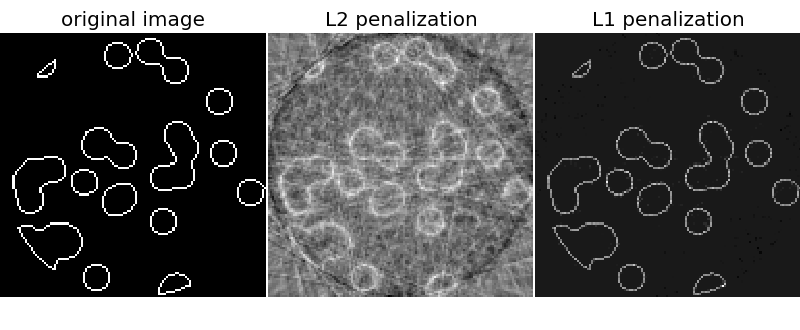
\includegraphics[width = \linewidth]{plot_tomography_l1_reconstruction_001.png}
        	\end{column}\hfill
        	\begin{column}{.25\textwidth}
        		EEG\\
        		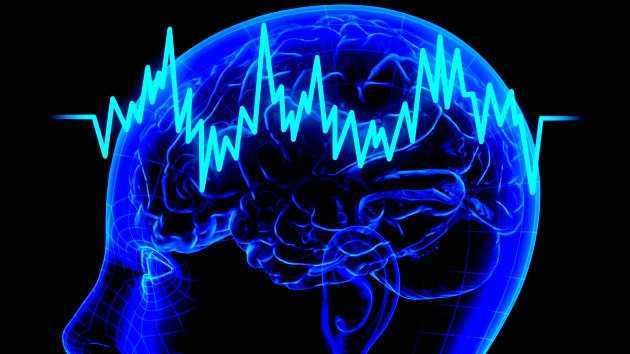
\includegraphics[width = \linewidth]{eeg_pic.jpg}
        	\end{column}\hfill
        	\begin{column}{.25\textwidth}
        		Image Reconstruction\\
        		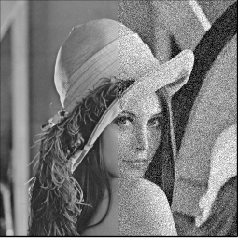
\includegraphics[width = \linewidth]{lena_pic.jpg}
        	\end{column}
        \end{columns}
  \end{frame}

  \begin{frame}\frametitle{ML and Optimization I}
    \alert{Training} a Machine Learning model means finding optimal parameters $\omega$:

    $$ \omega^* = \argmin_{\omega} F(\omega, X, z)$$
    \pause
    \begin{itemize}
      \item \alert{$F$}: Loss function of chosen ML-model
      \item \alert{$X$}: The training data ($N:=\#$samples $\times$ $\#$features matrix)
      \item \alert{$z$}: Training labels (only in classification models; vector of size $N$)
      \pause
      \item The dimension $n$ of $\omega$ is model dependent, often $\#$features$+1$
    \end{itemize}   
  \end{frame}

  \begin{frame}\frametitle{ML and Optimization II}
    After we have found $\omega^*$, we can do \alert{Prediction} on new data points:

    $$ \hat {z_i} := h(\omega^*, x_i)$$
    \pause
    \begin{itemize}
      \item \alert{$x_i$}: new data point with \emph{unknown} label \alert{$z_i$}
      \item \alert{$h$}: hypothesis function of the ML model
    \end{itemize}   
  \end{frame}

  \begin{frame}
    \frametitle{Challenges in Machine Learning}
      \begin{itemize}
        \item Massive amounts of training data 
        \item Construction of very large models
        \item Handling high memory/computational demands
      \end{itemize}
      \vspace{36pt}
      \pause
    \centering \large{Ansatz: \alert{Stochastic Methods}}
  \end{frame}
  
  \begin{frame}{Stochastic Framework}
    $$ F(\omega) := \mathbb{E}\left[f(\omega, \xi)\right] \uncover<3>{= \frac{1}{N}\sum_{i=1}^N f(\omega, x_i, z_i)}$$
    \begin{itemize}
      \item<2-> \alert{$\xi$}: Random variable; takes the form of an input-output-pair $(x_i, z_i)$
      \item<3-> \alert{$f$}: Partial loss function corresponding to a single data point.
    \end{itemize}
  \end{frame}

  \begin{frame}{Stochastic Methods}
    \begin{columns}[T]
      \begin{column}{.5\textwidth}
        \centering \alert{Gradient Method}
        $$\min F(\omega) $$

        \uncover<2->{
        $$\omega^{(k+1)}:= \omega^{(k)}-\alpha_k \nabla F(\omega^{(k)})$$\\
        \phantom{zeile}
        }
      \end{column}\hfill
      \begin{column}{.5\textwidth}
        \centering \alert{Stochastic Gradient Descent}
        $$\min \mathbb E \left [f(\omega, \xi)\right]$$
        \uncover<3>{
          $$\omega^{(k+1)}:= \omega^{(k)}-\alpha_k \alert{\nabla \hat F(\omega^{(k)})} $$
          with
          $$\alert{\nabla \hat F(\omega^{(k)})} := \frac{1}{b}\sum_{i\in \mathcal S_k}f(\omega, x_i, z_i)$$
          where $\mathcal S_k \subset [N], \quad b:=|\mathcal S_k| \ll N$\\\alert{"Mini Batch"}
        }
      \end{column}
    \end{columns}
  \end{frame}

\section{SQN: A Stochastic Quasi-Newton Method}
 \plain{Classification\\
 	\vspace{10pt}
 	\alert{Did we just detect a Higgs-Boson?}
 	\vspace{15pt}\\
 	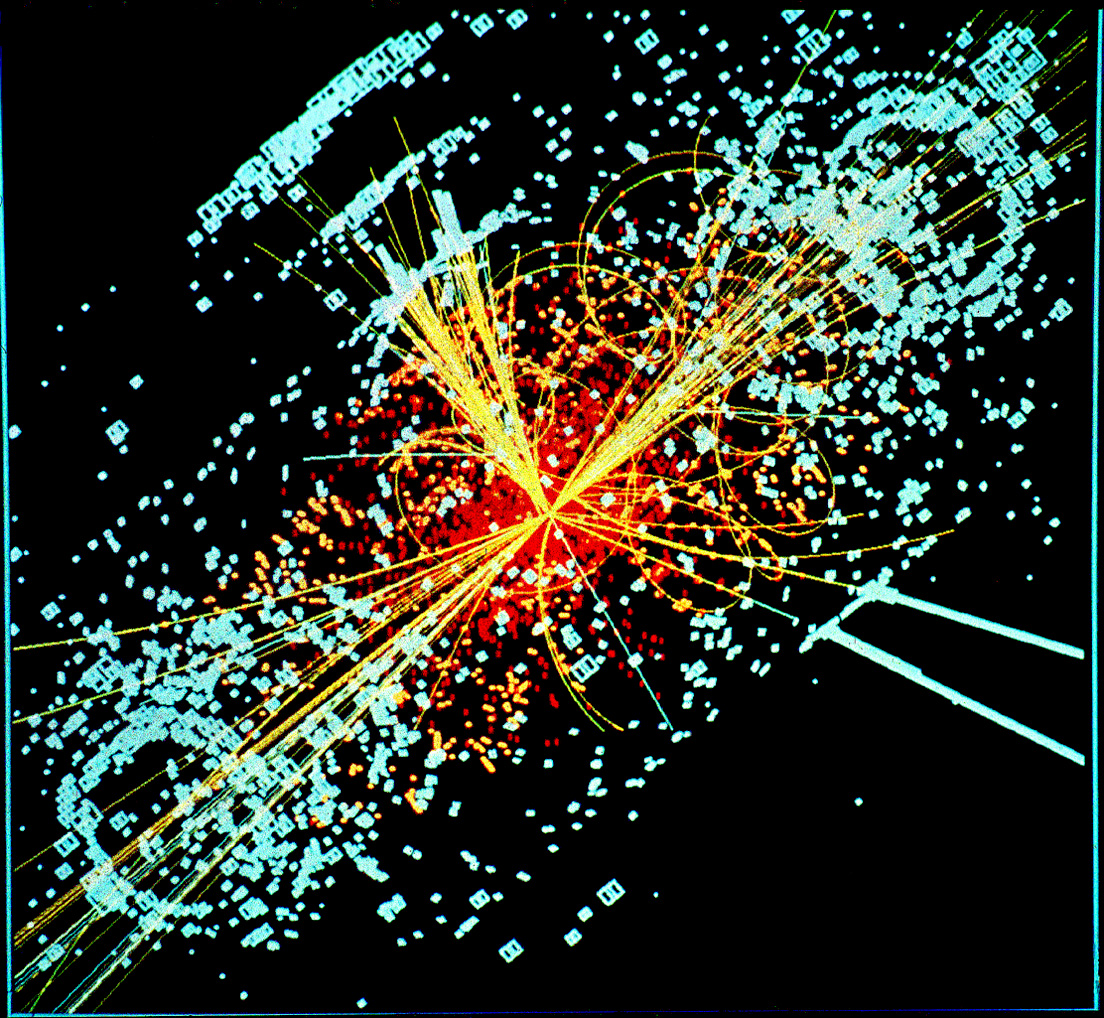
\includegraphics[width = 0.5\textwidth]{CMS_Higgs-event.jpg}}

  \begin{frame}
    \frametitle{Higgs-Boson classification problem}
      \begin{itemize}
        \item Data from Monte-Carlo simulations
        \item $X\in \mathbb R^{11.000.000 \times 29}$\\\emph{Lots} of samples, relatively small, dense feature set.
        \item Here, we use \emph{Logistic Regression} for classification.
      \end{itemize}
  \end{frame}

  \begin{frame}\frametitle{Stochastic Quasi-Newton Method (SQN)}
      \begin{itemize}
        \item \alert{Stochastically} use second-order information
        \item Based on BFGS-method.
        \pause
        \item Basic idea: $$ \omega^{(k+1)} = \omega^{(k)} - \alpha_k \alert{H_t} \nabla \hat F(\omega^{(k)})$$
        \pause
        \item $t$ running on slower time-scale than $k$. 
        \item $H_t$ update in $\mathcal O(n)$ time and constant memory, using several tricks
      \end{itemize}
  \end{frame}


  \begin{frame}
    \frametitle{Behavior}
      Pretty picures about the behaviour of SQN on HIGGS
      and comparison with traditional SGD
  \end{frame}

  \begin{frame}\frametitle{Results}
    \begin{itemize}
      \item Can be faster than SGD on appropriate Datasets
      \item Requires tedious, manual tuning of hyperparameters to be efficient!
    \end{itemize}
  
  \end{frame}

 \section{Proximal Method}
 \plain{Image Reconstruction\\
 	\vspace{10pt}
 	\alert{What did the original image look like?}
 	\vspace{15pt}\\
 	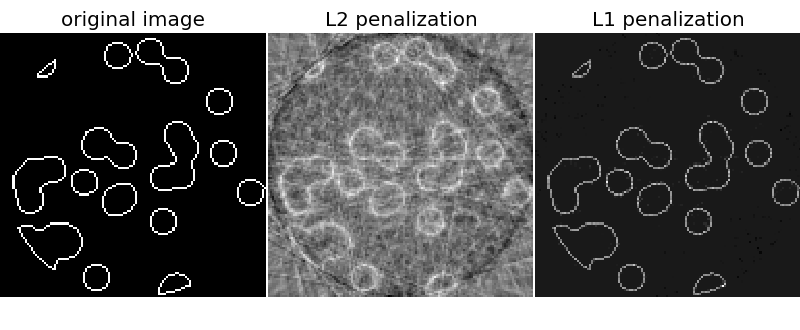
\includegraphics[width = 0.8\textwidth]{plot_tomography_l1_reconstruction_001.png}}
 
 
   \begin{frame}\frametitle{Proximal Method}
       \begin{flalign*}
       	\text{\alert{Problem}}&&
       	\min_x &\;F(x) := \underbrace{f(x)}_{smooth} \quad + \underbrace{h(x)}_{non-smooth}&
       \end{flalign*}
       \pause
       \begin{flalign*}
       	\text{\alert{Proximity Operator}}&&\prox_f(v) = &\underset{x}{\argmin} \; \bigl( f(x) + \frac{1}{2} \lVert x - v \rVert^2_2 \bigr)&
       \end{flalign*}
			\centering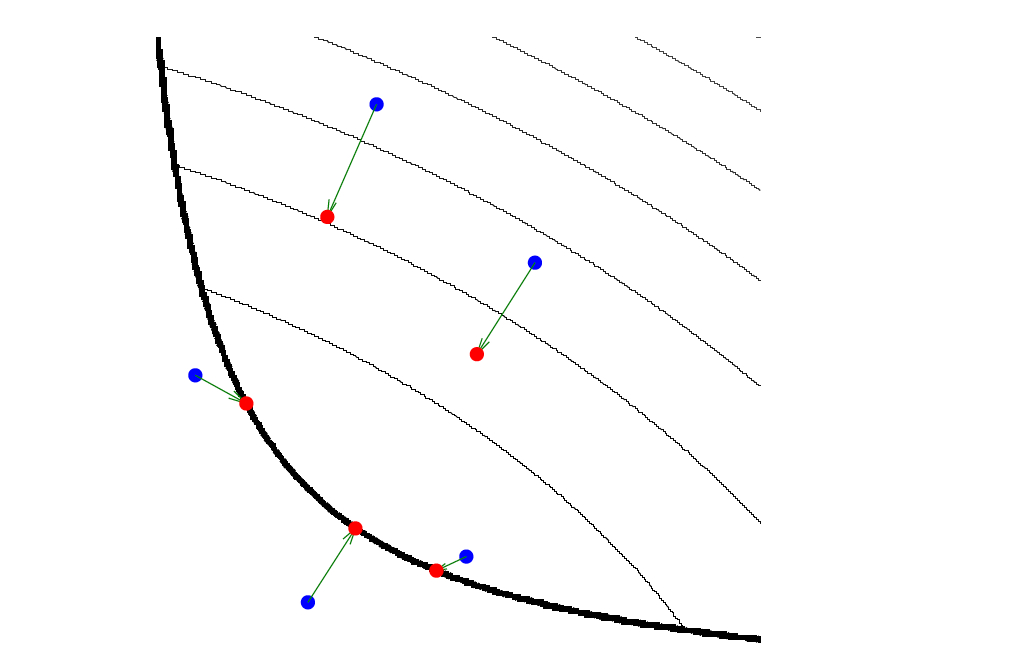
\includegraphics[width = 0.5\textwidth]{prox_boyd.jpg}
   \end{frame}
   
   \begin{frame}{Proximal Method}
   	\alert{Traditional Proximal Gradient Step:}
   	\begin{equation*}
   	x_{k+1} = \prox_{\lambda_kh}(x_k - \lambda_k\nabla f(x_k))
   	\end{equation*}
   	\alert{Quasi-Newton Proximal Step:}
   	\begin{equation*}
   	x_{k+1} = \prox_h^{B_k}(x_k - B_k^{-1}\nabla f(x_k)),
   	\end{equation*}
   	with $B_k = \underbrace{D_k}_{diag} + \underbrace{u_k}_{\in\mathbb{R}^n}u_k^T$.
   \end{frame}
   
   \begin{frame}{Proximal Method}
   	\begin{columns}[T]
   		\begin{column}{.5\textwidth}
   			$F(x) = \lVert Ax - b \rVert + \lambda \lVert x \rVert_1$\\
   			$A \in \mathbb{R}^{1500 \times 3000},\:b \in \mathbb{R}^{1500}$\\
   			$A_{ij},\:b_i\:$ \textasciitilde $\:\mathcal{N}(0,1)$, $\:\lambda = 0.1$\\
   			\vspace{10pt}
   			\resizebox{\linewidth}{!}{% This file was created by matplotlib v0.1.0.
% Copyright (c) 2010--2014, Nico Schl�mer <nico.schloemer@gmail.com>
% All rights reserved.
% 
% The lastest updates can be retrieved from
% 
% https://github.com/nschloe/matplotlib2tikz
% 
% where you can also submit bug reports and leavecomments.
% 
\begin{tikzpicture}

\begin{axis}[
xlabel={Number of Iterations},
ylabel={Function Value},
xmin=0, xmax=55,
ymin=10, ymax=10000000000000,
ymode=log,
axis on top,
legend entries={{0SR1},{ProxGrad},{L-BFGS-B}}
]
\addplot [thick, red]
coordinates {
(0,23930.000884189)
(1,2334714540827.73)
(2,1603.06839363472)
(3,1004.45275331694)
(4,588.495767390219)
(5,2465.40475724742)
(6,179.594821649387)
(7,126.10021752328)
(8,61.4875604431263)
(9,129.281440688095)
(10,45.4082629909795)
(11,42.394874463473)
(12,119.624730091399)
(13,51.1689226777425)
(14,32.9092659784772)
(15,29.0693418166155)
(16,56.3092645316347)
(17,42.3296301168754)
(18,26.0389860835202)
(19,24.072093333035)
(20,29.9753713640302)
(21,34.7565678982828)
(22,21.2930785912614)
(23,20.2111387939323)
(24,27.3668342566393)
(25,19.5107974611296)
(26,18.4848613019356)
(27,18.2334402824762)
(28,18.3815429335346)
(29,18.8034834674539)
(30,17.87043345129)
(31,17.8003210729537)
(32,18.0911346039328)
(33,17.8675588710352)
(34,17.6897872539639)
(35,17.657870704215)
(36,17.7868354702454)
(37,17.6638138927485)
(38,17.6029421873073)
(39,17.5857582401889)
(40,17.593531318576)
(41,17.6173728315327)
(42,17.5451975095162)
(43,17.5349437987365)
(44,17.5463738339233)
(45,17.5615379779338)
(46,17.5098254996569)
(47,17.502148251481)
(48,17.5255046093324)
(49,17.51125728217)
(50,17.4770773904264)
(51,17.4669089400231)
(52,17.4917281760979)
(53,17.4651780471754)
(54,17.446393502165)
(55,17.4367726172038)

};
\addplot [thick, blue]
coordinates {
(0,23930.000884189)
(1,7180.45388604586)
(2,3617.86527996726)
(3,2206.80793392946)
(4,1491.00767628939)
(5,1073.99586354884)
(6,808.278854547473)
(7,628.014922400163)
(8,499.960644278589)
(9,405.752764676303)
(10,334.52634655712)
(11,279.477813847677)
(12,236.164491398145)
(13,201.577684383878)
(14,173.611856832551)
(15,150.754899712087)
(16,131.896367104543)
(17,116.20926011348)
(18,103.06516983272)
(19,91.9789779656275)
(20,82.5721972749523)
(21,74.5480919899652)
(22,67.6703468931341)
(23,61.7492516151206)
(24,56.6308080266971)
(25,52.1895417181108)
(26,48.3230738518772)
(27,44.9473811889776)
(28,41.9908958545994)
(29,39.3943307887263)
(30,37.1076648133911)
(31,35.0895582332656)
(32,33.3047098499916)
(33,31.7230458561848)
(34,30.3185369243055)
(35,29.0691392036425)
(36,27.9557168948839)
(37,26.9619473758925)
(38,26.0735819006833)
(39,25.2785051309949)
(40,24.5658953302441)
(41,23.9261996677162)
(42,23.3512128923731)
(43,22.8338555363931)
(44,22.3679803523897)
(45,21.9478508869475)
(46,21.5686369463874)
(47,21.2260325999356)
(48,20.9161983824383)
(49,20.6357394037178)
(50,20.3816052485759)
(51,20.1511846245288)
(52,19.942073913322)
(53,19.7522963849272)
(54,19.5798157329886)
(55,19.4229051369124)

};
\addplot [thick, green!50.0!black]
coordinates {
(0,23930.000884189)
(1,12083.1529253535)
(2,1962.70076992746)
(3,950.485602345173)
(4,331.959633328347)
(5,243.914762566925)
(6,134.329835058351)
(7,101.908974098636)
(8,71.430490269532)
(9,53.8008057292489)
(10,49.2070909809805)
(11,47.2377989642264)
(12,45.8394992598531)
(13,44.9246042975355)
(14,44.7440629754329)
(15,44.39329787842)
(16,44.3236229723654)
(17,44.2184239820041)
(18,44.1931882049634)
(19,44.1267629597911)
(20,44.1051433432534)
(21,44.0736620641302)
(22,44.0227863049802)
(23,43.9604053846835)
(24,43.8383240409788)
(25,43.7012466950384)
(26,43.4900906898139)
(27,43.1528664627698)
(28,42.5004315629993)
(29,41.8013543791512)
(30,40.8296742339329)
(31,39.900023272227)
(32,38.5823534699433)
(33,37.4156430458995)
(34,36.2719668390337)
(35,35.0776601950381)
(36,34.1837687644875)
(37,33.2698645775237)
(38,32.1962015032741)
(39,31.3082549503913)
(40,30.4262826422634)
(41,29.5345560514281)
(42,28.6995811800974)
(43,27.8507440638526)
(44,26.8903832876716)
(45,26.0249848856949)
(46,25.0716863775733)
(47,24.1555764755733)
(48,23.4070450974266)
(49,22.7049953977644)
(50,22.0172886765464)
(51,21.3371046021488)
(52,20.6002987471974)
(53,19.9394587462096)
(54,19.3137752887323)
(55,18.6682287336718)
(56,18.1127667913341)

};
\path [draw=black, fill opacity=0] (axis cs:13,1)--(axis cs:13,1);

\path [draw=black, fill opacity=0] (axis cs:1,13)--(axis cs:1,13);

\path [draw=black, fill opacity=0] (axis cs:13,0)--(axis cs:13,0);

\path [draw=black, fill opacity=0] (axis cs:0,13)--(axis cs:0,13);

\end{axis}

\end{tikzpicture}}
   		\end{column}\hfill
   		\begin{column}{.5\textwidth}
   			$F(x) = \lVert Ax - b \rVert + \lambda \lVert x \rVert_1$\\
   			$A \in \mathbb{R}^{1500 \times 3000},\:b \in \mathbb{R}^{1500}$\\
   			$A_{ij},\:b_i\:$ \textasciitilde $\:\mathcal{N}(0,1)$, $\:\lambda = 0.1$\\
   			\vspace{10pt}
   			\resizebox{\linewidth}{!}{% This file was created by matplotlib v0.1.0.
% Copyright (c) 2010--2014, Nico Schl�mer <nico.schloemer@gmail.com>
% All rights reserved.
% 
% The lastest updates can be retrieved from
% 
% https://github.com/nschloe/matplotlib2tikz
% 
% where you can also submit bug reports and leavecomments.
% 
\begin{tikzpicture}

\begin{axis}[
xlabel={Number of Iterations},
ylabel={Function Value},
xmin=0, xmax=55,
ymin=10, ymax=10000000000000,
ymode=log,
axis on top,
legend entries={{0SR1},{ProxGrad},{L-BFGS-B}}
]
\addplot [thick, red]
coordinates {
(0,23930.000884189)
(1,2334714540827.73)
(2,1603.06839363472)
(3,1004.45275331694)
(4,588.495767390219)
(5,2465.40475724742)
(6,179.594821649387)
(7,126.10021752328)
(8,61.4875604431263)
(9,129.281440688095)
(10,45.4082629909795)
(11,42.394874463473)
(12,119.624730091399)
(13,51.1689226777425)
(14,32.9092659784772)
(15,29.0693418166155)
(16,56.3092645316347)
(17,42.3296301168754)
(18,26.0389860835202)
(19,24.072093333035)
(20,29.9753713640302)
(21,34.7565678982828)
(22,21.2930785912614)
(23,20.2111387939323)
(24,27.3668342566393)
(25,19.5107974611296)
(26,18.4848613019356)
(27,18.2334402824762)
(28,18.3815429335346)
(29,18.8034834674539)
(30,17.87043345129)
(31,17.8003210729537)
(32,18.0911346039328)
(33,17.8675588710352)
(34,17.6897872539639)
(35,17.657870704215)
(36,17.7868354702454)
(37,17.6638138927485)
(38,17.6029421873073)
(39,17.5857582401889)
(40,17.593531318576)
(41,17.6173728315327)
(42,17.5451975095162)
(43,17.5349437987365)
(44,17.5463738339233)
(45,17.5615379779338)
(46,17.5098254996569)
(47,17.502148251481)
(48,17.5255046093324)
(49,17.51125728217)
(50,17.4770773904264)
(51,17.4669089400231)
(52,17.4917281760979)
(53,17.4651780471754)
(54,17.446393502165)
(55,17.4367726172038)

};
\addplot [thick, blue]
coordinates {
(0,23930.000884189)
(1,7180.45388604586)
(2,3617.86527996726)
(3,2206.80793392946)
(4,1491.00767628939)
(5,1073.99586354884)
(6,808.278854547473)
(7,628.014922400163)
(8,499.960644278589)
(9,405.752764676303)
(10,334.52634655712)
(11,279.477813847677)
(12,236.164491398145)
(13,201.577684383878)
(14,173.611856832551)
(15,150.754899712087)
(16,131.896367104543)
(17,116.20926011348)
(18,103.06516983272)
(19,91.9789779656275)
(20,82.5721972749523)
(21,74.5480919899652)
(22,67.6703468931341)
(23,61.7492516151206)
(24,56.6308080266971)
(25,52.1895417181108)
(26,48.3230738518772)
(27,44.9473811889776)
(28,41.9908958545994)
(29,39.3943307887263)
(30,37.1076648133911)
(31,35.0895582332656)
(32,33.3047098499916)
(33,31.7230458561848)
(34,30.3185369243055)
(35,29.0691392036425)
(36,27.9557168948839)
(37,26.9619473758925)
(38,26.0735819006833)
(39,25.2785051309949)
(40,24.5658953302441)
(41,23.9261996677162)
(42,23.3512128923731)
(43,22.8338555363931)
(44,22.3679803523897)
(45,21.9478508869475)
(46,21.5686369463874)
(47,21.2260325999356)
(48,20.9161983824383)
(49,20.6357394037178)
(50,20.3816052485759)
(51,20.1511846245288)
(52,19.942073913322)
(53,19.7522963849272)
(54,19.5798157329886)
(55,19.4229051369124)

};
\addplot [thick, green!50.0!black]
coordinates {
(0,23930.000884189)
(1,12083.1529253535)
(2,1962.70076992746)
(3,950.485602345173)
(4,331.959633328347)
(5,243.914762566925)
(6,134.329835058351)
(7,101.908974098636)
(8,71.430490269532)
(9,53.8008057292489)
(10,49.2070909809805)
(11,47.2377989642264)
(12,45.8394992598531)
(13,44.9246042975355)
(14,44.7440629754329)
(15,44.39329787842)
(16,44.3236229723654)
(17,44.2184239820041)
(18,44.1931882049634)
(19,44.1267629597911)
(20,44.1051433432534)
(21,44.0736620641302)
(22,44.0227863049802)
(23,43.9604053846835)
(24,43.8383240409788)
(25,43.7012466950384)
(26,43.4900906898139)
(27,43.1528664627698)
(28,42.5004315629993)
(29,41.8013543791512)
(30,40.8296742339329)
(31,39.900023272227)
(32,38.5823534699433)
(33,37.4156430458995)
(34,36.2719668390337)
(35,35.0776601950381)
(36,34.1837687644875)
(37,33.2698645775237)
(38,32.1962015032741)
(39,31.3082549503913)
(40,30.4262826422634)
(41,29.5345560514281)
(42,28.6995811800974)
(43,27.8507440638526)
(44,26.8903832876716)
(45,26.0249848856949)
(46,25.0716863775733)
(47,24.1555764755733)
(48,23.4070450974266)
(49,22.7049953977644)
(50,22.0172886765464)
(51,21.3371046021488)
(52,20.6002987471974)
(53,19.9394587462096)
(54,19.3137752887323)
(55,18.6682287336718)
(56,18.1127667913341)

};
\path [draw=black, fill opacity=0] (axis cs:13,1)--(axis cs:13,1);

\path [draw=black, fill opacity=0] (axis cs:1,13)--(axis cs:1,13);

\path [draw=black, fill opacity=0] (axis cs:13,0)--(axis cs:13,0);

\path [draw=black, fill opacity=0] (axis cs:0,13)--(axis cs:0,13);

\end{axis}

\end{tikzpicture}}
   		\end{column}
   	\end{columns}
   \end{frame}
   
   \begin{frame}{Proximal Method}
   	\alert{Effect of regularization parameter $\lambda$ on solution:}\\
   	\centering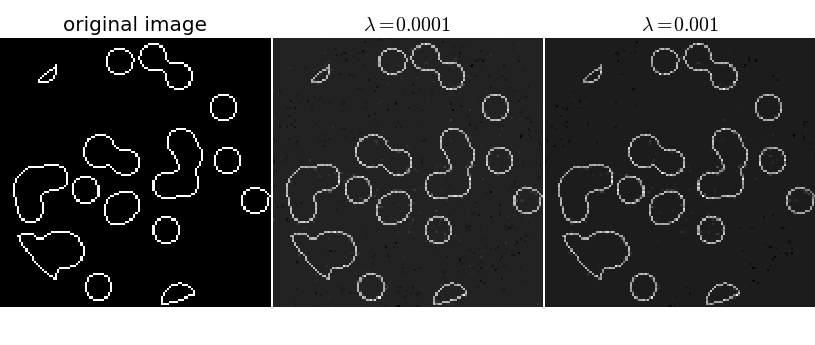
\includegraphics[width = 0.7\textwidth]{lambda1.png}\\
   	\centering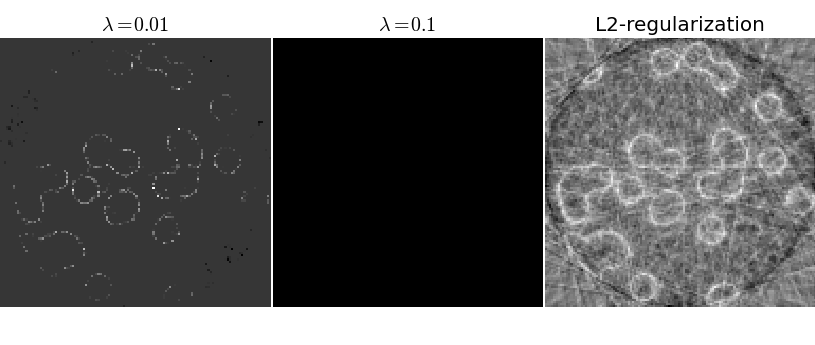
\includegraphics[width = 0.7\textwidth]{lambda2.png}
   \end{frame}

\section{Logistic Regression: An Example}
  \begin{frame}\frametitle{Task}
    Explain what we want to do, and explain the dataset,
    and why using both SQN and Prox makes sense   
  \end{frame}

  \begin{frame}\frametitle{Results}
    Nice table with SQN, SGD (no reg, L2), (Lasso,) Prox (L1) showing
    Obj. value in found optimum, CPU time, Iterations, F1 score of prediction model

    \begin{table}[t]
    \centering
      \begin{tabular}{r|c|c|c}
        \phantom 0 & \textbf{$F(\omega^*)$} & \textbf{Model Score} & \textbf{Cost}\\
      \hline \alert{No regularization}   &      & &  \\
        SGD   & $0.01$  & $96\%$  & $x$ sec, $y$ AP\\
        SQN   & $0.5$  & $96\%$  & $x$ sec, $y$ AP\\
        Prox   & $0.01$  & $96\%$  & $x$ sec, $y$ AP\\
      \hline \hline \alert{L1}        &    &   &  \\
      LASSO & $.71$  &  $55\%$ & blablabla \\
        Prox   & $0.01$  & $96\%$  & $x$ sec, $y$ AP\\
      \hline \hline \alert{L2}        &    &   &  \\
       SGD & $.71$  &  $55\%$ & blablabla \\
        SQN   & $0.01$  & $96\%$  & $x$ sec, $y$ AP\\
      \end{tabular}
    \end{table}
  \end{frame}

\plain{
  \resizebox{\textwidth}{!}{    
      \begin{tabular}{r|c|c|c}
        \phantom 0 & \textbf{$F(\omega^*)$} & \textbf{Model Score} & \textbf{Cost}\\
      \hline \alert{No regularization}   &      & &  \\
        SGD   & $0.01$  & $96\%$  & $x$ sec, $y$ AP\\
        SQN   & $0.5$  & $96\%$  & $x$ sec, $y$ AP\\
        Prox   & $0.01$  & $96\%$  & $x$ sec, $y$ AP\\
      \hline \hline \alert{L1}        &    &   &  \\
      LASSO & $.71$  &  $55\%$ & blablabla \\
        Prox   & $0.01$  & $96\%$  & $x$ sec, $y$ AP\\
      \hline \hline \alert{L2}        &    &   &  \\
       SGD & $.71$  &  $55\%$ & blablabla \\
        SQN   & $0.01$  & $96\%$  & $x$ sec, $y$ AP\\
      \end{tabular}
      }
    
    }

\section{Conclusion}

  \begin{frame}{Summary}
    \begin{center}\ccbysa\end{center}
  \end{frame}
  

  \plain{Questions?}

  \begin{frame}[allowframebreaks]\frametitle{Main References}

    \bibliography{refs}
    \bibliographystyle{abbrv}

  \end{frame}

\end{document}
